\chapter{EVENT LOCALIZATION}
 \label{chap:eventLo}
\section{Introduction}
This section of thesis considers the problem of localization: the objective is to detect where an action of interest occurs. The expected output of such a system is typically a subvolume encompassing the action of interest. Since a localized action only covers a fraction of the spatio-temporal volume in a video, the task is considerably more challenging than event classification. Some of the common startergies that are tried on this kind of problems are efficient sub-window search ~\citep{subwindowsearch},"selective search" stratergy ~\citep{selectivesearch}  and a recent by ~\cite{tubelet}, but these either does a exhaustive search or does a iterative merging of the supervoxels. 

\section{Background Subtraction Techniques} 
\par Event localization can be performed by determining the position with pixel changes and understanding the motion relativity ~\citep{Basharat08}, where all components corresponding to an event show a similar flow of pixels. Following approach works significantly well in surveillance data but fails terribly in case human event detection. Later realized that, by eliminating the background(static parts) of the visual frame,  possible event locations can be retained.  Several background subtraction technique are eminent in the \cite{Piccardi04}, among these some apply on static image while others on dynamic video. In case of our application we can blend both these approaches to generate more reliable event detectors.

\subsection{Frame Differencing (FD)}
A very common approach for performing the moving object segmentation is using frame differencing but these approach is very sensitive to small changes and yields lots of noise when a camera is in motion. A simplest way to implement this technique is by computing the absolute difference of gray scale/intesity values two consecutive frames. Consider $P(p_x,p_y,t)$, intesity of pixel $(p_x,p_y)$ at frame t, then pixel $(p_x,p_y)$ that is considered foreground when absolute difference is above a threshold,$$\vert P(p_x,p_y,t+1) - P(p_x,p_y,t)t\vert > T$$.
\par The robustness of this method depends on speed of forground elements. Faster movements may require higher thresholds to reduce the noise.  An alternate approach is to replace difference of a single previous frame  by an average of multiple previous frames, still results are noisy and not reliable.

\subsection{Mixture of Gaussian (MOG)}
This is one of the well known method of extracting foreground information. \cite{kaew} model each background pixel by a mixture of N Gaussian distributions. The weights of the mixture represent the time proportions that those colors stay in the scene. The probable background colors are the ones which stay longer and more static. At any instance $i$ a particular pixel $(p_x,p_y)$ has color space represented as $V(p_{x},p_{y},i)$, history of the pixels are given by 
$$X_{1},..,X_{t} = {V(p_{x},p_{y},i)~:~1\le i \le t }$$
The history is modeled by mixture of N gaussian mixtures,
$$P(X_{t})=\Sigma_{i}^{N}w_{i,t}\eta(X_{t}|\mu_{i,t},\Sigma_{i,t})$$
\par $w_{i,t}$, $\mu_{i,t}$, $\Sigma_{i,t}$ are weight,mean and covariance of the $i^{th}$ Gaussian in the mixture at time $t$ respectively and where $\eta$ is gaussian density function. General principle behind this approach is that when a new object occludes the background object, it will not match one of the existing distributions. Instead will result in either the creation of a new distribution or the increase in the variance of an existing distribution. The variance of the moving object is expected to remain larger than a background pixel until the moving object stops.


\subsection{Eigen subtraction (ES)}
An alternate approach named eigen background subtraction was seen to be more elegant. A sample of N images of the videos are obtained, mean background image $\nu_b$ is computed and all images are mean normalized  $X$. Principal component analysis on the mean normalized images is performed , idea is, that a high-dimensional images are often described by correlated variables and only a few meaningful dimensions account for most of the information. But performing PCA is not straightforward, consider 100 images of dimension 100x100 pixels, then the dimension of generated covariance matrix would be 10000x10000, i.e roughly 0.8 GB (considering 64 bit float values). Solving this is not feasible, hence a trick from linear algebra that for a MXN matrix with $M>N$, can at most have N-1 non-zero eigen values ~\cite{Duda01} can be used. Eigen decomposition of $X^TX$ is carried out:
$$X^TX\nu_i=\lambda_i\nu_i$$
$$XX^T(X\nu_i)=\lambda_i(X\nu_i)$$
The orthonormal eigen vector of $XX^T$ is found out by normalizing $X\nu_i$ to unit length. Once eigen vectors of $XX^T$  are computed, projection of the current frame $F$ on the eigen vector with top eigen values are determined, and the reconstructed frame $F'$ is obtained by using the projection coefficients and the eigen vectors. The difference $F-F'$ would correspond to the mask on the moving object. 

\begin{figure}[htpb]
   \begin{center}
	    \includegraphics[width=0.75\textwidth]{snaps/bgsub/results.eps}     
     \caption {Background subtraction techniques on multiple video classes}
   \label{fig:bgsub}
   \end{center}
 \end{figure}
\par Results of foreground mask obtained using FD, ES and MOG are shown in Figure \ref{fig:bgsub}. Eventhough MOG is most preferred, but found it provide sparse and not a clear boundary in most of the sample videos. In the example of "dance", the FD yields extraneous pixels due to camera movemnet in between two dancers, which are not evident in ES and MOG. While it produces spurious pixels for the "pommello" video, because of sharp background. All methods terribly fail incase of grainy videos, hence background subtraction alone cant be suffice for the event localization.

\section{Saliecny Detection}
Visual saliency is the distinct subjective perceptual quality which makes some items in the world stand out from their neighbors and immediately grab our attention.
As we had discussed earlier about the different techniques to extract the eminent pixels which are in motion, sometimes pixels which are stationary and quite distinct might also play a important role in the the activity recognition. These approaches are considered during the process attention modelling. Most of saliency estimations techniques follow the following five steps which can be visualized in Figure \ref{fig:salap},
\begin{itemize}
\item{\textbf{Step 1: Color equalization:} This is performed by removing the tail in the color histogram. It helps improving the contrast in the image. In the implmentation color equalization is done on each channel separetely so that all channels can be provided to the segmentation algorithm.}

\item{ \textbf{Step 2: SLIC-based segmentation:}  It is a simple linear iterative clustering that clusters pixels in the combined five-dimensional color and image plane space to efficiently generate compact, nearly uniform superpixels. Any slic based clustering algorithm takes two parameters number of super-pixels and compactness of each superpixel. According to \cite{slic}, slic is fastest and most memory efficient compared to  other segmentation technique like graph-cut, quick shift segmentation technques. Segmentation reduces the number of computation in the subsequent stages.}

\item{ \textbf{Step 3: Extract segment properties:} Extracting features of the region that are used in computing the saliecny of each regions. Some features that are considered in the implementation are color based features (LAB,RGB) and texture based features (GLCM,Texture Flow).}

\item{\textbf{Step 4: Compute~saliency:} Saliecny estimation techniques can be broadly categorized into bottom-up, top-down and information maximization based on algorithmic computation. Earliest saliency based attention modelling was proposed by \cite{itti}. It was inspired by the behavior and the neuronal architecture of the early primate visual system.}

\item{\textbf{Step 5: Saliency cut:} Saliency maps are generally thresholded to obtain the salient mask. In the implementation, grab-cut\citep{grabcut} performs segmentation by modeling foreground and background based on saliency estimation to obtain the mask where higher saliency  contemplate foreground while lower saliency estimate corespond to background. Once saliency mask are obtained few morphological operation are applied to remove the salt and pepper noise.}
\end{itemize}

\begin{figure}[htpb]
   \begin{center}
	    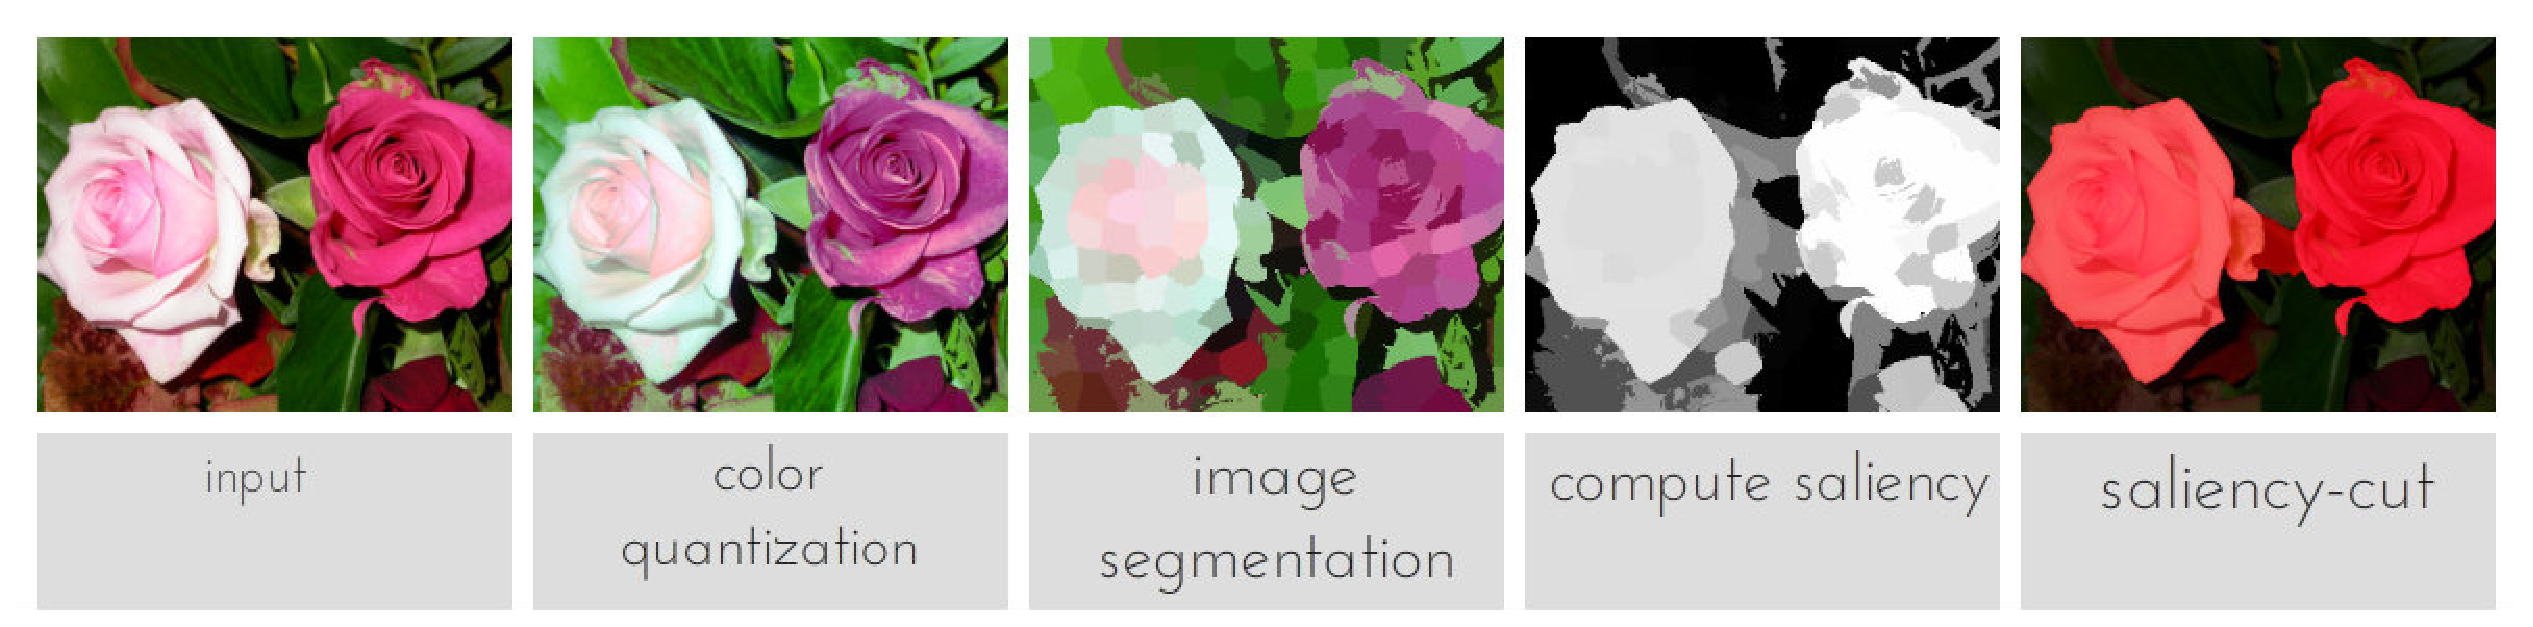
\includegraphics[width=0.95\textwidth]{snaps/sal/saliency.eps}     
     \caption {A general approach for saliency estimation}
   \label{fig:salap}
   \end{center}
 \end{figure}

\par Some of the saliency estimation techniques that were studied in the thesis are discussed below. All these techniques can be considered at region level or pixel level, based on whether the segmentation of the image is considered or not.

\subsection{Hierarchical Color Based (HCB)}
HCB is a top-down approach for computing saliency where saliency map of improbable pixels/regions are set to zero at every iteration. Saliency of pixel/region $I_{x}$ is computed by folowing formulation. 
$$ Iavg_{x} = \Sigma_{y} I_{y}~\exp^{-\frac{\parallel~p_{x} - p_{y}~\parallel}{w}}  $$
$$ saliency(I_{x}) =~\parallel I_{x} - Iavg_{x} \parallel $$
where $p_{x}$ is the position of the pixel $I_{x}$. At each iteration, the $w$ is decreased implying closer neigborhood. After each iteration we eliminate pixels/regions with $ saliency(I_{x})$ lesser than $0.1$ after normalization. In this manner, we  discard the background pixels/regions leaving out only the foreground pixels/regions. The main focus of this technique is to measure the variation from the average pixel intensity.

\subsection{Context Aware Based (CAB)}
In CAB, saliency estimate are averaged out at a different context windows. The expressions for the estimation of saliency is given below,
$$ AllPairDistance(I_{x},I_{y},k) = \exp^{-\frac{\parallel~p_x - p_y~\parallel}{dw_k}}~\exp^{-\frac{\parallel~I_{x} - I_{y}~\parallel}{cw}}$$
$$ NormDistance(I_{y},k) = \Sigma_{x} AllPairDistance(I_{x},I_{y},k)$$
$$ saliency(I_{x}) = 1- \Sigma^{K}_{k=1}~dw_{k}~\Sigma_{y}~\frac{AllPairDistance(I_{x},I_{y},k)}{NormDistance(I_{y},k)}$$
where $cw$ and $K$ are color weight and number of context windows respectively. Saliency measures the similarity with its neighborhood weighted on proximity of the pixels/regions. $AllPairDistance(I_{x},I_{y},k)$ is disparity measure across pairs of pixels/regions $(I_{x},I_{y})$ for different values of $dw_{k}$ while $NormDistance(I_{y},k)$ correspond to the normalizing factor.
This technique perform fairly well in discriminating saliency objects which are not in same scale.

\subsection{Spectral Distribution Based (SDB)} 
SDB is based on the intuition that pixels with small color distribution variances have high saliency values. The extent color distribution is measured by color spatial variance. \cite{spectralSal} proposed a technique to compute color spatial variances using Gaussian Mixture Models (GMMs). All pixels/regions in the image are represented by GMMs using Expectation Maximization (EM) algorithm, where $w_{c}$, $\mu_{c}$ $\Sigma_{c}$ is the weight, the mean color, and the covariance matrix of the $c^{th}$ mixture. Each pixel/region is assigned to a mixture with the probability:
$$p(c | I_{x}) = \frac{w_{c}\eta(I_{x}| \mu_{c},\Sigma_{c})}{\Sigma_{c}w_{c}\eta(I_{x}| \mu_{c},\Sigma_{c}} $$
Suppose $x_{h}$ is the x coordinate (horizontal coordinate) of the pixel x. The spatial variance for x-dimension of color component c is computed as:
$$\sigma_{h}^{2}(c) = \frac{1}{|P|_{c}}\Sigma_{x}	p(c | I_{x}) \parallel x_{h} -M_{h}(c) \parallel^{2}$$
where $M_{h}(c) = \frac{1}{|P|_{c}}\Sigma_{x}p(c|I_{x})~x_h$ , and $|P|_{c} = \Sigma_{x}p(c | I_{x})$ is a normalization factor. The vertical variance $\sigma_{v}^{2}(c)$ is defined similarly. The spatial variance of a component c is combined as: $\sigma^{2}(c) = \sigma_{h}^{2}(c) + \sigma_{c}^{2}(c)$ which is then normalized.
The saliency $saliency(I_{x})$ of a specific pixel $I_{x}$ regarding to color spatial
distribution is defined as the weighted sum:
$$saliency(I_{x}) = \Sigma_{x}p(c | I_{x})(1-\sigma^{2}(x))$$
This method yields very good results for many examples but the configurations requires tweaks for better results.

\subsection{Regional Contrast (RC)}
RC evaluates saliency of an image region using its contrast with respect to the entire image. Several approaches  \citep{globContrast}, {patchRarities}, \citep{salFilters} for computing saliency based on global contrast are known in literature while in this work, these techniques are fused and presented as solitude.
It considers two contrast measures:
\subsubsection{Uniqueness}
Element uniqueness is contemplated with  assumption that image regions, which stand out from other regions in certain aspects, catch our attention and hence to be labeled more salient. Element uniqueness for segment $I_{x}$, given its position $p_{I_{x}}$ compared to all other $I_{y}$ is defined as follows,
$$uniqueness(I_{x}) = \Sigma_{y} \parallel~I_{x} -I_{y}~\parallel~\exp^{-\frac{\parallel~p_{x} - p_{y}~\parallel}{dw}}$$
where $dw$ controls the proximity of the neigborhood, higher value correspond to wider neigborhood.
\subsubsection{Distribution}
In general, colors belonging to the background will be distributed over the entire image exhibiting a high spatial variance, whereas foreground objects are generally more compact. Element distribution measure for a segment $I_{x}$ using the spatial variance of its color as follows,
$$distribution(I_{x}) = \Sigma_{y} \parallel~p_{y} -\mu_{x}~\parallel~\exp^{-\frac{\parallel~I_{x} - I_{y}~\parallel}{cw}}$$ 
where $\mu_{x} = \Sigma_{y}~p_{y}~exp^{-\frac{\parallel~I_{x} - I_{y}~\parallel}{cw}}$, measures weighted mean position of the color of $I_{x}$ component. Low variance indicates a spatially compact object hence they are considered more salient than spatially widely distributed elements.

\par The two above contrast measures defined at element level can be conolidated by given expression,
$$saliency(I_{x}) = uniqueness(I_{x}) \exp^{-k~distribution(I_{x})}$$
where $k$ controls the empasis on distribution while both the contrast measure are normalized. It is observed that the uniqueness performs well in case of single object saliency while for multiple object saliency, uniqueness together with distribution yields better result. Saliency mask obtained using HCB, CAB, SDB and RC for some standard weizmann segmentation dataset images are shown in Figure \ref{fig:sal}. 

\begin{figure}[htpb]
   \begin{center}
	    \includegraphics[width=0.75\textwidth]{snaps/sal/saliencyall.eps}     
     \caption {Saliency mask obtained using multiple techniques}
   \label{fig:sal}
   \end{center}
 \end{figure}

 \section{Smoothening}
Smoothening of the mask obtained at frame level is essential because of the occlussion and illumination variations. All the approaches were implemented by considering a context before and after the frame. A common approach which was followed for the smoothening of frame was by blending the background subtraction measure and the saliency measure to obtain a visual attention score. Higher visual attention score ($\geqslant0.8$) were considered \textsc{True Foreground} while lower visual attention score ($\leqslant0.2$)  were considered \textsc{True Background}. Then models are built for prediction of other regions/pixels. Three approaches for smoothening of visual attention measure are demonstrated below,
\subsection{Eigen Based}
Eigen Based method is based on projecting the pixels along the direction of maximum variance for foreground and background. Any pixel is assigned foreground if the projection along the direction of maximum variance for foreground is larger compared to  background. The direction of maximum variance are computed by gathering features (pixel level features like color, texture, gradient and position) of forground/background pixels in the context and perform the principal compoenent analysis (PCA). But this approach of smoothening, has been failing in most of the scenarios and did not yield good localization of event.
\subsection{Semi-supervised}
As all know semi-supervised learning is a situation where the training data some of the samples are not labeled. Hence the semi-supervised learning seems most appropriate for the smoothening task, as it would make use of the unlabeled data to capture the manifold of the underlying data distribution and generalize better for new examples. In this thesis, label proagation \citep{labprop}, a graph based semi supervised learning was materialized for polishing the mask. This technique was computationally intensive as we required to build model using all pixels in the frame in given context.There was no sort of adaptation mechanism which was available, for a faster convergence of learning algorithm.
\subsection{Guassian Mixture Based}
Gaussian mixture model was  most successful experiment among the techniques considered.  In this approach, two gaussian mixture model were built using true foreground and background  examples. Each and every pixels are assigned to either forground or background based on the likelihood scores of foreground and background model . One of the biggest advantage of this approach is its support to adapt, i.e models of previous frames can be finetuned for the current frames which helps training individual context models quickly.
\par Among all the methods the gaussian mixture models are considered for all the experiments because of its swiftness and the robustness. Few post processing operation were carried over the predicted mask like median blurring,region filling were done to remove the salt and pepper noises and spurious regions that are puny. Figure \ref{fig:smoothen}  shows obtained smoothened mask using different techniques from the visual attention score.
\section{Tracking}
 
\section{Summary}
